\documentclass[conference]{IEEEtran}

\usepackage{amsmath}
\usepackage{amssymb}
\usepackage{booktabs}
\usepackage{balance}
\usepackage{graphicx}
\usepackage{multirow}
\usepackage{url}
\usepackage[hidelinks]{hyperref}
\usepackage{xcolor}

\graphicspath{{../figures/publication/}}

\begin{document}

\title{Auditing an Interpretable Weather--Symptom--Disease Cascade:
Leakage-Resistant Evaluation and Error Propagation}

\author{
\IEEEauthorblockN{
Yun Tao, Sijie Liu, Junhan Yi, Yumeng Jin, Yinuo Pang}
\IEEEauthorblockA{
\textit{Artificial Intelligence Programme}\\
\textit{Beijing Normal--Hong Kong Baptist University}\\
Zhuhai, Guangdong, China}
}

\maketitle

\begin{abstract}
Semantic bottlenecks can make machine-learning pipelines easier to inspect,
but their end-to-end value depends on whether the intermediate concepts can be
predicted reliably. We audit a two-stage weather--symptom--disease cascade on
the public Weather-related Disease Prediction Dataset. The released file
contains 5,200 rows, 219 of which are exact duplicates; one of 37 symptom
columns is constant. Our primary analysis therefore uses 4,981 unique rows and
36 estimable symptoms. We construct a locked, weather-signature-disjoint test
set (3,984 development and 997 test rows), generate five-fold group-disjoint
out-of-fold symptom predictions for disease-stage training, and select all
thresholds without test-label access. On the locked test set, weather-only
XGBoost attains a symptom micro-F1 of 0.1889. The best direct weather-only
disease model reaches 20.16\% accuracy (95\% bootstrap confidence interval
[17.75\%, 22.67\%]), close to the 19.36\% class-prior baseline, whereas the
prespecified XGBoost-to-TabNet cascade reaches 11.94\%
[10.03\%, 13.94\%]. Adding age, gender, and documented pre-existing
conditions raises direct XGBoost accuracy to 41.12\%
[38.01\%, 44.03\%]; a context-aware XGBoost symptom bottleneck followed by
XGBoost reaches 39.62\% [36.61\%, 42.73\%]. In contrast, TabNet supplied with
true symptoms reaches 96.29\% [95.09\%, 97.39\%]. The resulting
84.35-percentage-point Oracle-to-deployable gap identifies intermediate
prediction error as the dominant limitation. The cascade is thus a useful
model-audit case study, but the present data do not support clinical,
causal, or early-warning claims. External validation with patient identifiers,
timestamps, locations, and independent outcomes is required.
\end{abstract}

\begin{IEEEkeywords}
clinical prediction model audit, semantic bottleneck, error propagation,
weather and health, multilabel classification, calibration, reproducibility
\end{IEEEkeywords}

\section{Introduction}

Weather and climate exposures are associated with substantial health burden,
including heat-related mortality and changes in infectious and respiratory
risk \cite{vicedo2021}. Machine learning can represent nonlinear relations
among environmental, demographic, and health variables, but apparent
predictive performance may be misleading when duplicate records, non-independent
splits, in-sample intermediate predictions, or weak baselines are not handled
explicitly.

A semantic bottleneck offers an intuitively attractive design. Instead of
mapping weather directly to a disease label, a first model predicts named
symptoms, and a second model maps the symptom representation to disease.
Humans can inspect the intermediate concepts, and the two stages can be
diagnosed separately. This interpretability argument, however, is not itself a
performance guarantee. If weather carries little information about individual
symptoms, the second stage receives a noisy representation and may underperform
a direct classifier.

This study revises and audits such a two-stage cascade. The audit was motivated
by three questions:

\begin{enumerate}
    \item Can weather variables predict the released symptom labels under a
    group-disjoint, leakage-resistant protocol?
    \item Does the predicted-symptom bottleneck improve disease classification
    over direct and class-prior baselines?
    \item How much of the end-to-end error is attributable to the symptom
    prediction layer rather than the disease classifier?
\end{enumerate}

Our contributions are methodological rather than clinical. We provide a
checksum-verified data pipeline, remove exact duplicates, make units explicit,
train the disease stage on out-of-fold predictions, lock the final test set,
report uncertainty and calibration, and compare predicted, thresholded, true,
and context-enriched symptom representations. The audit finds a large gap
between true and predicted symptoms. This negative result is scientifically
important: semantic interpretability is meaningful only when the intermediate
concepts are observable or predictable at the intended decision time.

\section{Related Work and Reporting Standards}

\subsection{Weather, health, and prediction}

Attribution research has established that human-induced climate change has
already increased heat-related mortality \cite{vicedo2021}. Such population-level
associations motivate environmental health forecasting, but they do not imply
that a small set of contemporaneous weather measurements can diagnose an
individual disease. Prediction tasks must distinguish population risk,
surveillance, and individual diagnosis, because each requires different
outcomes, sampling frames, and validation designs.

\subsection{Semantic bottlenecks and tabular models}

Concept bottleneck models explicitly predict human-defined concepts before a
final task, enabling intervention and inspection at the concept layer
\cite{koh2020}. Our symptom layer has this structure, although the public data
do not provide concept annotations with timing or clinical adjudication.
XGBoost is a regularized gradient-boosting implementation effective for
heterogeneous tabular predictors \cite{chen2016}. TabNet uses sequential
attention to select tabular features and provides instance-level feature masks
\cite{arik2021}. We treat these algorithms as model families to be evaluated,
not as evidence of clinical validity.

\subsection{Transparent prediction-model evaluation}

TRIPOD+AI emphasizes transparent reporting of data sources, participants,
predictors, outcomes, analysis, performance, and limitations for prediction
models using regression or machine learning \cite{collins2024}. PROBAST+AI
similarly structures risk-of-bias and applicability assessment
\cite{moons2025}. Following these principles, we report duplicate handling,
units, split independence, missing metadata, baselines, confidence intervals,
calibration, and the precise boundary between internal benchmarking and
external validation.

\section{Data and Audit Findings}

\subsection{Source and provenance}

We use version 1 of the Weather-related Disease Prediction Dataset, published
on Zenodo under CC BY 4.0 \cite{shan2024}. The archived CSV is preserved
unchanged and verified before each publication run with the official MD5
checksum:
\texttt{4aa51b2bb76b45b2000ce71517a0fd1e}.

The file contains age, binary gender, temperature in degrees Celsius, humidity,
wind speed in km/h, binary symptom and pre-existing-condition indicators, and
an 11-class \texttt{prognosis} label. The diseases are arthritis, common cold,
dengue, eczema, heart attack, heat stroke, influenza, malaria, migraine,
sinusitis, and stroke.

\begin{table}[t]
\caption{Data audit and primary split}
\label{tab:data}
\centering
\begin{tabular}{lr}
\toprule
Item & Count/value\\
\midrule
Released rows / columns & 5,200 / 51\\
Exact duplicate rows & 219\\
Primary analysis rows & 4,981\\
Development / locked test rows & 3,984 / 997\\
Disease classes & 11\\
Source / modeled symptom columns & 37 / 36\\
Unique raw-weather signatures & 3,588\\
Weather-signature overlap across split & 0\\
Test rows sharing a symptom signature with development & 960\\
\bottomrule
\end{tabular}
\end{table}

\subsection{Data-quality decisions}

The source has no missing cells, but 219 rows are exact duplicates. The primary
analysis removes them before splitting. Two columns represent pain behind the
eyes with near-duplicate names; they are merged by row-wise maximum into one
concept. The \texttt{shivering} column is zero in all 5,200 rows, so its
positive-class performance is mathematically unidentifiable. It remains in the
data-quality inventory but is excluded from model fitting and macro averaging,
leaving 36 estimable symptoms.

Humidity values range from approximately 0.37 to 1.00. Although the archive
description calls humidity a percentage, we interpret the stored values as
fractions and convert them to percent only inside named meteorological
formulae. This decision is encoded once in the shared preprocessing function.

The source lacks patient identifiers, timestamps, locations, weather-station
identifiers, institutions, and cohort indicators. We therefore cannot verify
participant independence, temporal ordering, station matching, or geographic
separation. Table~\ref{tab:data} also shows that 960 of 997 test rows have a
symptom signature observed in development. The weather split prevents exact
weather-pattern leakage, but it cannot establish independent clinical
generalization. As a split-sensitivity diagnostic, a naive stratified row split
of the same size would share 280 raw-weather signatures between development
and test, covering 377 of 997 test rows; the primary grouped split reduces both
quantities to zero.

\section{Methods}

\subsection{Weather representations}

The raw weather representation is
$\mathbf{x}_{w}=(T,\mathrm{RH},v)$, where $T$ is temperature in
$^\circ$C, RH is relative humidity, and $v$ is wind speed in km/h. A full
weather representation appends four deterministic indices:

\begin{itemize}
    \item NOAA Rothfusz heat index, evaluated in Fahrenheit and converted back
    to Celsius in its warm--humid domain;
    \item humidex, using a Magnus dew-point approximation;
    \item Australian apparent temperature, converting wind to m/s; and
    \item temperature--humidity index
    \begin{equation}
    \mathrm{THI}=T-(0.55-0.0055\,\mathrm{RH})(T-14.5).
    \end{equation}
\end{itemize}

All transformations are deterministic. Scaling for logistic regression and
MLP models is fitted within the corresponding training fold only.

\subsection{Split, out-of-fold training, and thresholds}

We hash the three raw weather values to define a weather signature. A seeded
five-fold stratified group split contributes one fold as a locked test set and
the other four as development data. Identical raw-weather signatures therefore
cannot occur on both sides of the primary split. Within development, a second
five-fold stratified group split produces out-of-fold (OOF) symptom
probabilities.

For each symptom and Stage-1 model, the classification threshold is selected
using development OOF predictions only. The deployable disease-stage models
are fitted to OOF predicted symptom probabilities or OOF thresholded symptoms,
never to in-sample Stage-1 outputs. The locked test labels enter only the final
metric and statistical functions.

\subsection{Models and comparisons}

Stage 1 compares multilabel logistic regression (LR), a multilayer perceptron
(MLP), and XGBoost. Direct disease baselines include an empirical class-prior
classifier, multinomial LR, random forest (RF), MLP, and XGBoost. TabNet is the
prespecified primary Stage-2 model; LR, RF, MLP, and XGBoost are architecture
controls.

The experiments answer distinct questions:

\begin{enumerate}
    \item \textbf{Weather-only cascade:} weather $\rightarrow$ predicted
    symptoms $\rightarrow$ disease.
    \item \textbf{Binarization ablation:} symptom probabilities versus
    development-thresholded symptom indicators.
    \item \textbf{Direct baselines:} weather $\rightarrow$ disease.
    \item \textbf{Context extension:} age, gender, weather, and seven
    documented pre-existing conditions known before the modeled event.
    \item \textbf{Skip connection:} context concatenated with predicted
    symptom probabilities before disease classification.
    \item \textbf{Oracle upper bound:} true symptoms $\rightarrow$ TabNet.
\end{enumerate}

The context extension changes the scientific question: it evaluates pre-event
patient context plus weather, not weather alone. The Oracle is not deployable
at a pre-symptom decision time and is used only to localize the bottleneck.

\subsection{Metrics and statistical analysis}

Stage-1 metrics are micro- and macro-F1, micro- and macro-average precision
(AP), Hamming loss, and per-symptom precision, recall, F1, AP, prevalence, and
threshold. Disease metrics are accuracy, balanced accuracy, macro- and
weighted-F1, one-versus-rest macro AUROC and AP, negative log-likelihood,
multiclass Brier score, 10-bin expected calibration error (ECE), per-class
metrics, and confusion matrices.

We compute percentile 95\% confidence intervals for accuracy and macro-F1 with
2,000 seeded nonparametric bootstrap replicates \cite{efron1993}. Exact
McNemar tests compare paired locked-test correctness vectors
\cite{mcnemar1947}. Calibration is reported alongside discrimination because
low ECE alone can occur in an uninformative model that stays close to class
prevalence \cite{guo2017}.

\section{Results}

\subsection{Stage-1 symptom prediction}

Table~\ref{tab:stage1} reports locked-test symptom prediction. XGBoost on the
three raw weather variables has the highest weather-only micro-F1 (0.1939).
Appending deterministic weather indices does not improve XGBoost
(micro-F1 0.1889), suggesting that these transformations add little new
information. LR has the highest weather-only macro-F1 (0.1495) but lower
micro-AP. With pre-event context, XGBoost improves to micro-F1 0.2429 and
micro-AP 0.3754. Performance remains modest, so the semantic bottleneck is
noisy before disease-stage training begins.

\begin{table}[t]
\caption{Locked-test Stage-1 symptom performance}
\label{tab:stage1}
\centering
\resizebox{\columnwidth}{!}{
\begin{tabular}{llrrrr}
\toprule
Model & Inputs & Micro-F1 & Macro-F1 & Micro-AP & Hamming\\
\midrule
LR & Weather + indices & 0.1644 & 0.1495 & 0.1041 & 0.3843\\
MLP & Weather + indices & 0.1575 & 0.1225 & 0.0914 & 0.5356\\
XGBoost & Raw weather & \textbf{0.1939} & 0.1329 & 0.1616 & 0.2972\\
XGBoost & Weather + indices & 0.1889 & 0.1323 & 0.1587 & 0.3073\\
XGBoost & Full pre-event context & \textbf{0.2429} & \textbf{0.2436}
& \textbf{0.3754} & \textbf{0.2730}\\
\bottomrule
\end{tabular}}
\end{table}

\begin{figure}[t]
\centering
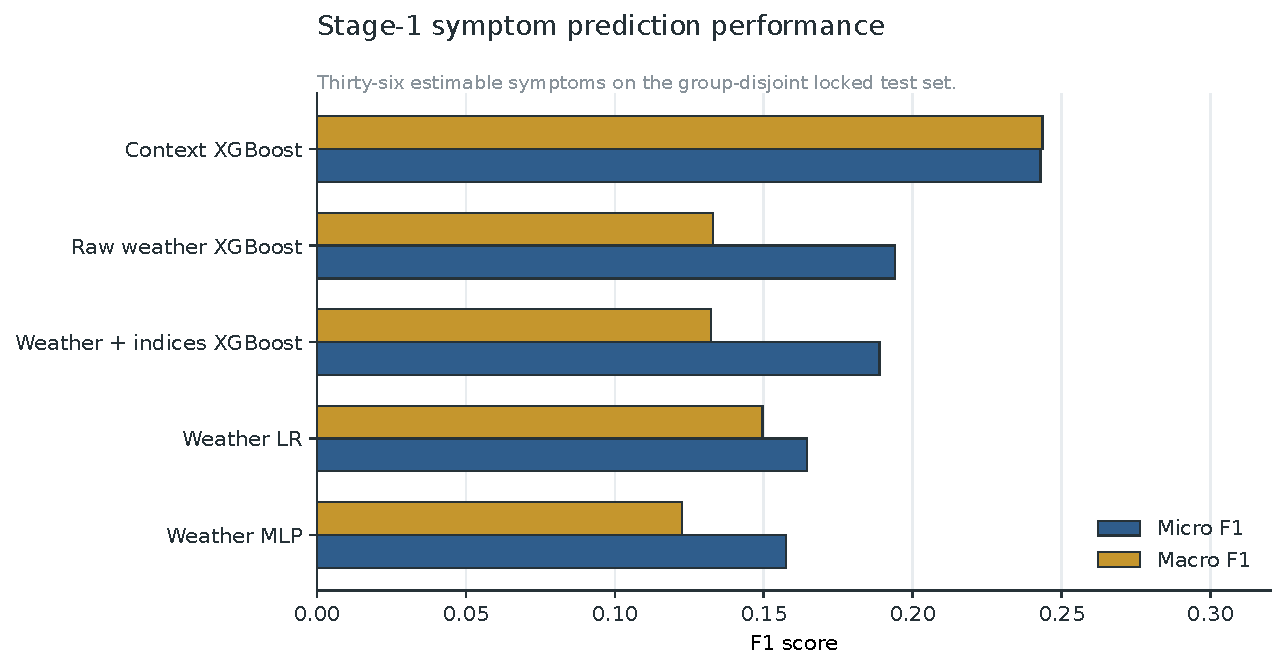
\includegraphics[width=\columnwidth]{Fig_Publication_Stage1_Performance.pdf}
\caption{Locked-test symptom prediction. The context extension is shown
separately because it changes the available information.}
\label{fig:stage1}
\end{figure}

\subsection{End-to-end disease classification}

Table~\ref{tab:endpoint} and Fig.~\ref{fig:endpoint} summarize the primary
endpoint. The empirical class-prior classifier reaches 19.36\% accuracy. The
best weather-only direct model is MLP at 20.16\%, with an interval overlapping
the prior baseline. The prespecified weather-only XGBoost-to-TabNet cascade
reaches 11.94\% and macro-F1 0.0470. It does not improve on the direct baseline.

\begin{table*}[t]
\caption{Locked-test disease classification ($n=997$)}
\label{tab:endpoint}
\centering
\begin{tabular}{p{3.7cm}p{3.7cm}ccc}
\toprule
System & Representation & Accuracy & 95\% CI & Macro-F1\\
\midrule
Class-prior baseline & Weather ignored & 19.36\% & [16.95, 21.77] & 0.0295\\
Direct MLP & Weather + indices & 20.16\% & [17.75, 22.67] & 0.0946\\
XGBoost $\rightarrow$ TabNet & Predicted symptoms, weather only
& 11.94\% & [10.03, 13.94] & 0.0470\\
Context XGBoost $\rightarrow$ TabNet & Context-predicted symptoms
& 25.78\% & [22.97, 28.49] & 0.1086\\
Context XGBoost $\rightarrow$ XGBoost & Context-predicted symptoms
& 39.62\% & [36.61, 42.73] & 0.2677\\
Skip connection XGBoost & Context + predicted symptoms
& 40.22\% & [37.21, 43.33] & 0.2744\\
Direct context XGBoost & Full pre-event context
& \textbf{41.12\%} & [38.01, 44.03] & \textbf{0.2865}\\
Oracle TabNet & True symptoms
& 96.29\% & [95.09, 97.39] & 0.9666\\
\bottomrule
\end{tabular}
\end{table*}

\begin{figure*}[t]
\centering
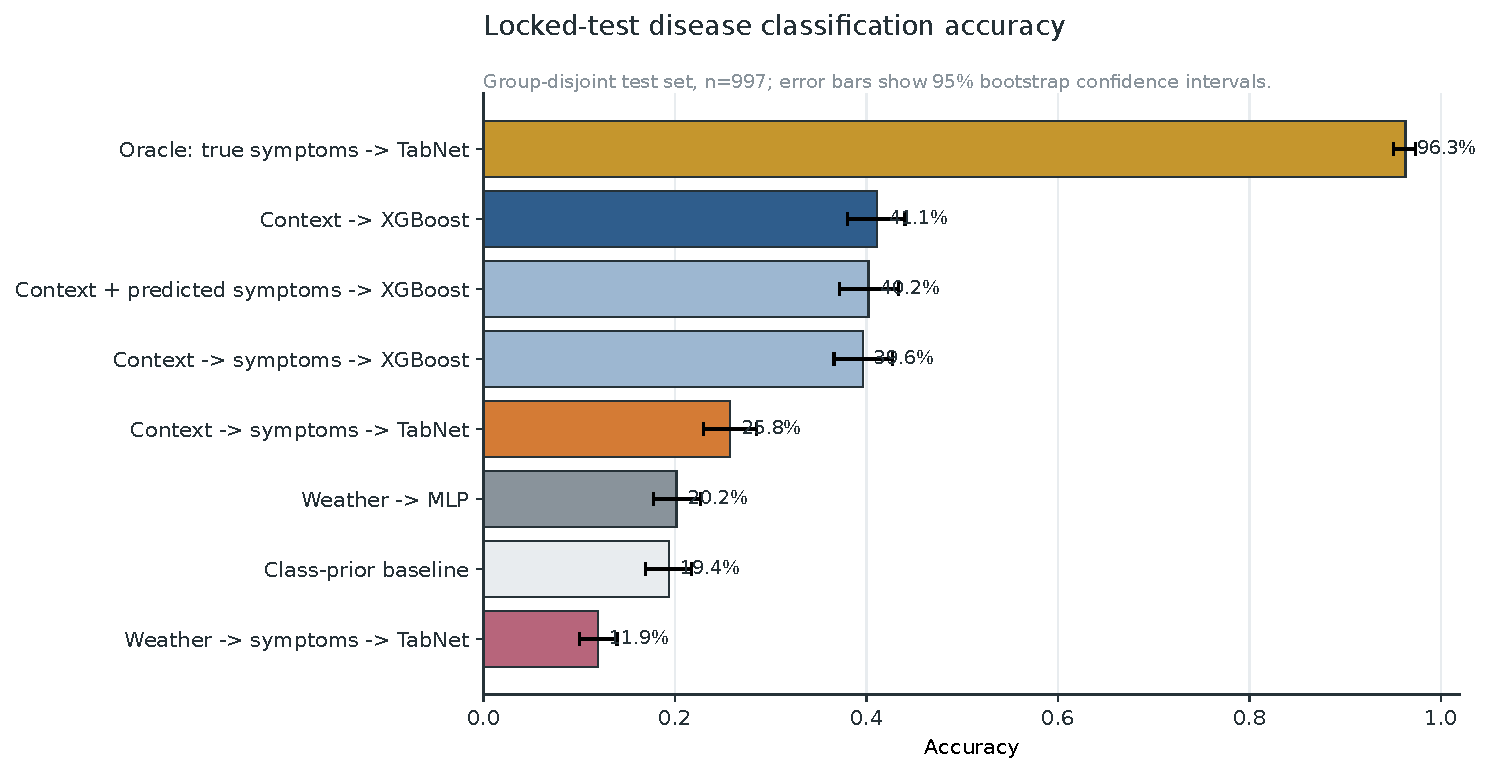
\includegraphics[width=0.90\textwidth]{Fig_Publication_Endpoint_Accuracy.pdf}
\caption{Locked-test accuracy with 2,000-replicate bootstrap confidence
intervals. Weather-only and context-extended experiments answer different
scientific questions; the Oracle is an upper bound, not a deployable model.}
\label{fig:endpoint}
\end{figure*}

The direct context model is numerically strongest among deployable systems
(41.12\%). A context-aware XGBoost-to-XGBoost bottleneck retains 39.62\%,
and a skip connection reaches 40.22\%. These small gaps show that a semantic
representation can retain much of the context model's endpoint accuracy when
both stages are matched to the tabular data, but it does not confer
superiority. The prespecified TabNet second stage is particularly sensitive to
noisy predicted symptom probabilities: replacing it with XGBoost raises the
context bottleneck from 25.78\% to 39.62\%.

For the weather-only primary cascade, direct XGBoost is correct on 154 test
rows where the cascade is wrong, whereas the cascade is correct on 93 rows
where direct XGBoost is wrong (exact McNemar $p=1.25\times10^{-4}$). Probability
and thresholded-symptom TabNet variants have identical accuracy and symmetric
discordance (98 versus 98; $p=1.0$), so the data do not establish superiority
of either representation. A non-significant test is not interpreted as
equivalence.

\subsection{Error propagation}

The Oracle TabNet reaches 96.29\% accuracy and macro-F1 0.9666. The same
disease-stage family supplied with weather-predicted XGBoost symptom
probabilities reaches only 11.94\%. The 84.35-percentage-point gap
(Fig.~\ref{fig:error}) demonstrates that the disease label is highly encoded
in the recorded symptom pattern, but that weather alone cannot reconstruct the
needed pattern in this evaluation.

\begin{figure}[t]
\centering
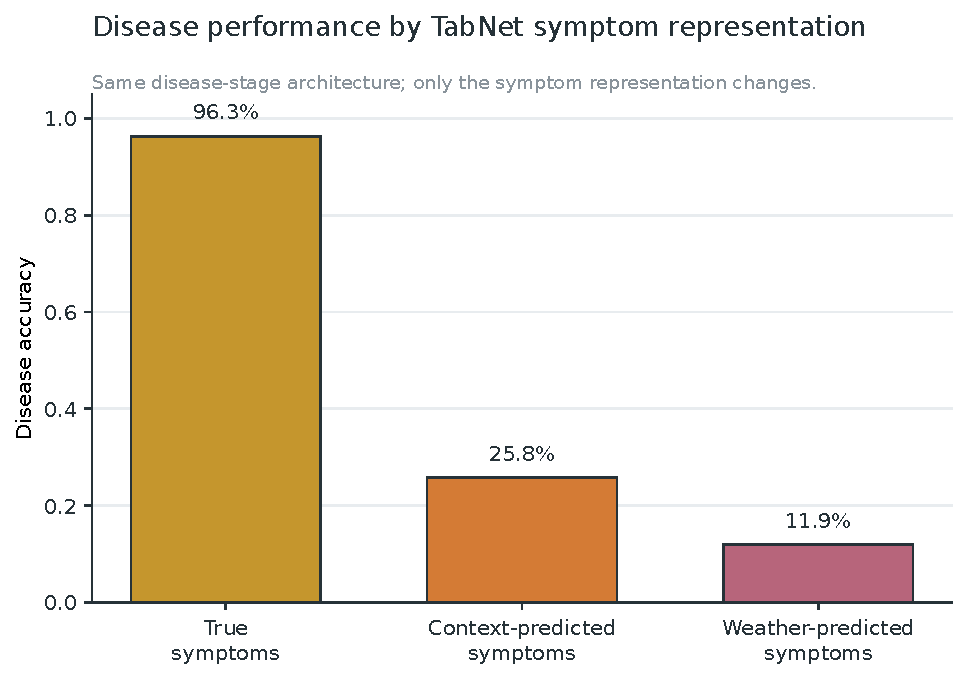
\includegraphics[width=\columnwidth]{Fig_Publication_Error_Propagation.pdf}
\caption{Error propagation when the same TabNet disease-stage architecture is
given weather-predicted, context-predicted, or true symptom representations.}
\label{fig:error}
\end{figure}

\subsection{Calibration, confusion, and attribution}

Figure~\ref{fig:calibration} plots confidence against observed accuracy. The
direct context XGBoost has ECE 0.0416; the context bottleneck with XGBoost has
ECE 0.0562. The weak weather-only TabNet cascade has ECE 0.0222, illustrating
why calibration error must not be read without accuracy and classwise
performance. The Oracle ECE is 0.1433 despite high accuracy, indicating that
its probability scale would still require calibration for any decision use.

\begin{figure}[t]
\centering
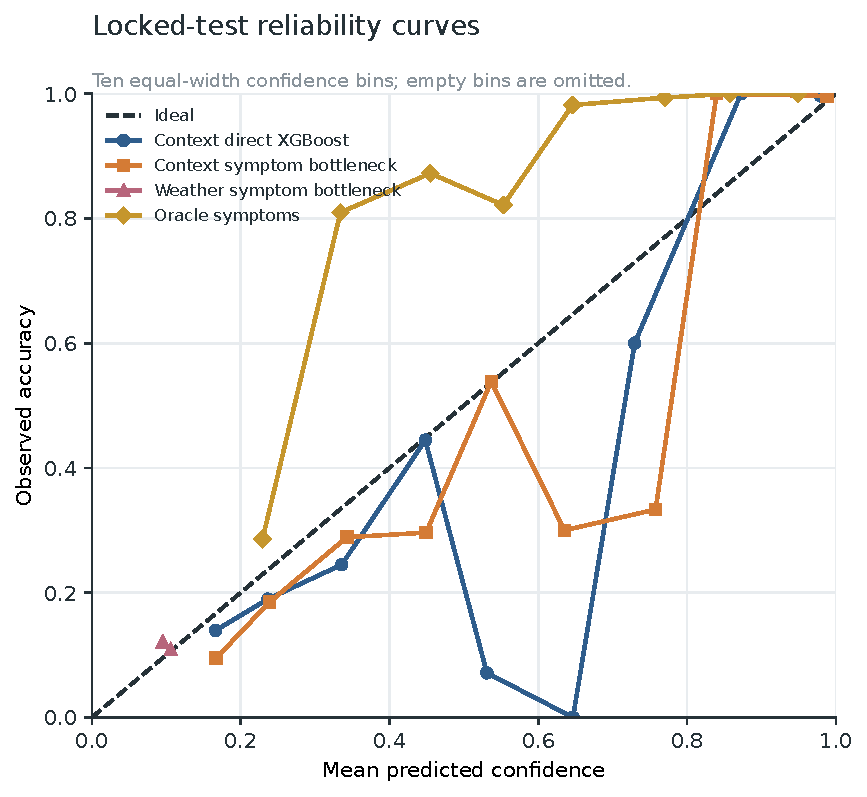
\includegraphics[width=\columnwidth]{Fig_Publication_Calibration.pdf}
\caption{Locked-test reliability curves. Marker area is proportional to bin
count; ECE is reported with, not instead of, discrimination metrics.}
\label{fig:calibration}
\end{figure}

The context symptom-bottleneck confusion matrix in
Fig.~\ref{fig:confusion} shows that a 39.62\% aggregate accuracy does not
translate to uniformly strong classwise recognition. This is reflected by the
lower macro-F1 of 0.2677.

\begin{figure}[t]
\centering
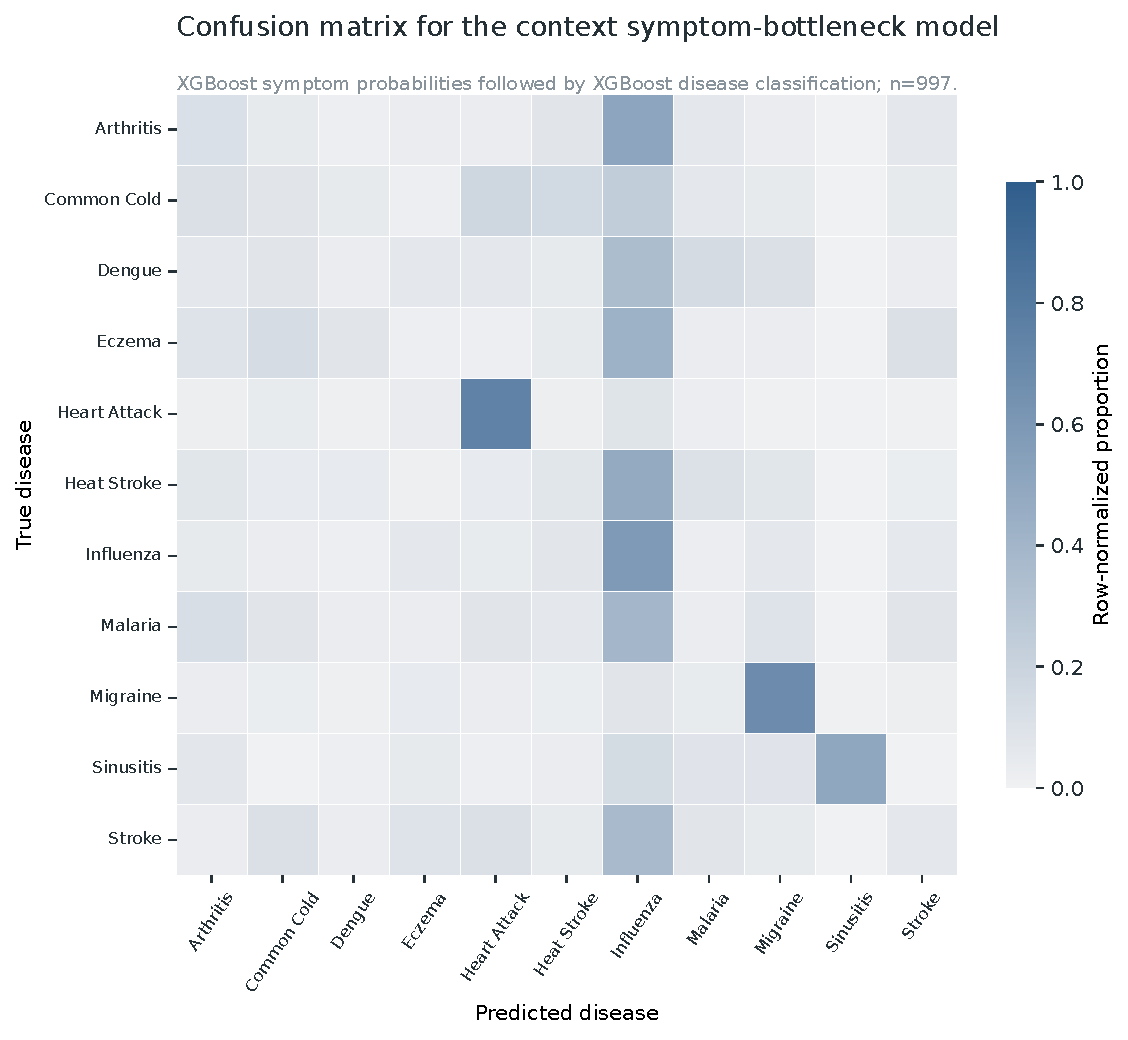
\includegraphics[width=\columnwidth]{Fig_Publication_Context_Confusion.pdf}
\caption{Row-normalized locked-test confusion matrix for context-predicted
XGBoost symptom probabilities followed by XGBoost disease classification.}
\label{fig:confusion}
\end{figure}

Permutation attribution is computed on held-out development-fold predictions,
not on the locked test set. For direct context XGBoost, high blood pressure,
HIV/AIDS, and nasal polyps have the largest macro-F1 decreases under
permutation. In the Stage-1 context model, high blood pressure and HIV/AIDS
dominate micro-AP importance. Aggregated TabNet masks in the Oracle model
emphasize headache, chest pain, high fever, pain behind the eyes, vomiting,
severe headache, rapid heart rate, and diarrhea
(Fig.~\ref{fig:importance}). These are associational model attributions, not
causal effects or clinical risk factors.

\begin{figure*}[t]
\centering
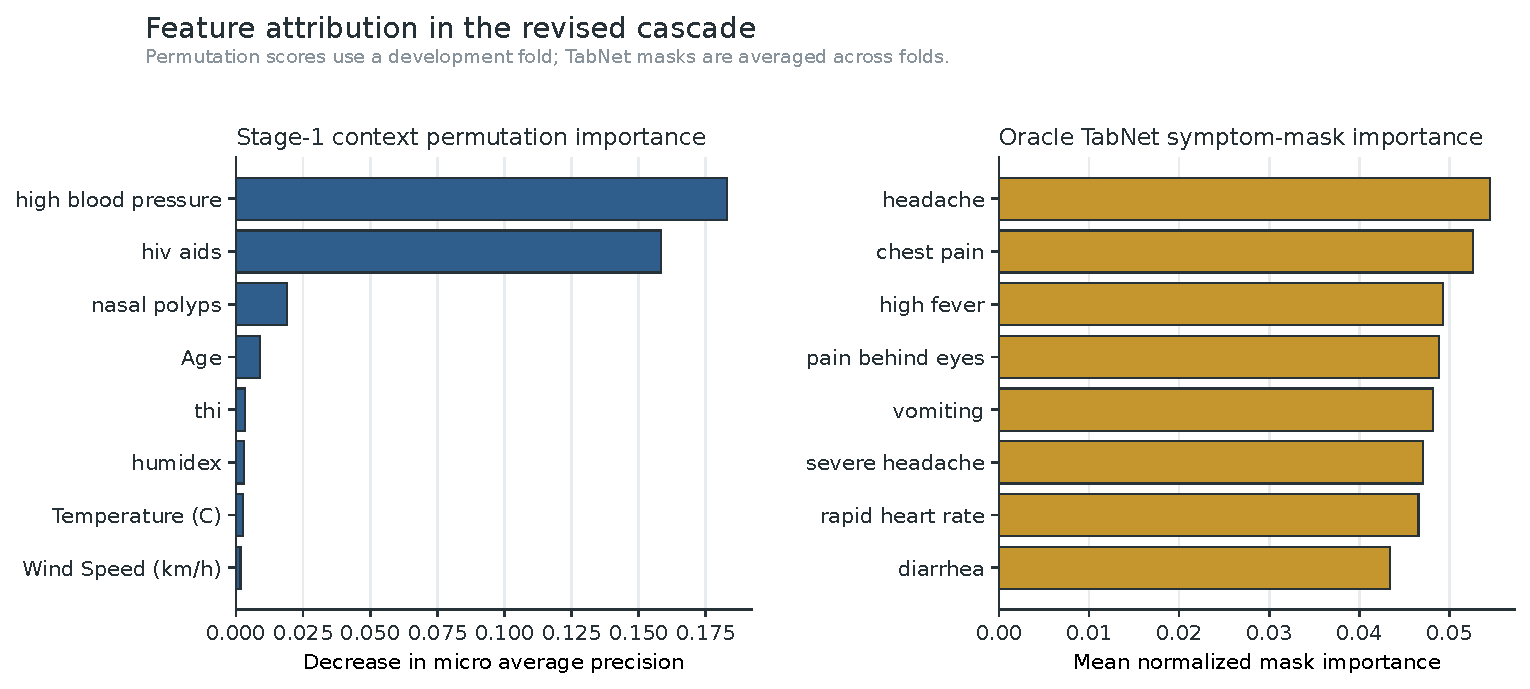
\includegraphics[width=0.95\textwidth]{Fig_Publication_Feature_Attribution.pdf}
\caption{Development-fold permutation importance for context models and
aggregated Oracle TabNet masks. Importance measures are model- and
representation-specific.}
\label{fig:importance}
\end{figure*}

\section{Discussion}

\subsection{What the audit changes}

The leakage-resistant results do not support the claim that three weather
measurements are sufficient for accurate individual disease prediction. The
best direct weather model is statistically compatible with a simple
class-prior baseline, and the prespecified deployable cascade performs below
that baseline. The more defensible contribution is an empirical account of
semantic-bottleneck error propagation.

The Oracle result is useful but easy to misuse. It shows that the recorded
symptoms nearly determine the released label under this split; it does not
show that those symptoms are available before diagnosis, independently
measured, or transferable to real clinical settings. Because 960 of 997 test
rows share a symptom signature with development, the Oracle may partly learn a
repeated label dictionary. It is an upper bound for this table, not a validated
diagnostic system.

\subsection{Interpretability--performance trade-off}

The symptom bottleneck makes the pipeline auditable: Stage-1 failure can be
separated from disease-stage failure, thresholds can be inspected, and the
effect of true versus predicted concepts can be quantified. With full
pre-event context and XGBoost at both stages, it retains most of the direct
model's endpoint accuracy. However, the bottleneck neither creates information
nor guarantees robustness. The skip connection recovers little beyond direct
context, and TabNet underperforms XGBoost when its inputs are noisy predicted
probabilities. Model architecture should therefore be matched to the
representation and validated empirically.

\subsection{Implications for additional experiments}

The highest-value next experiment is not another random internal split. It is
external validation on a temporally ordered cohort with patient, time,
location, station, and institution identifiers. Before accessing external
outcomes, the current feature construction, thresholds, and model
configurations should be frozen. The external study should report cohort flow,
missingness, class prevalence, distribution shift, subgroup performance, and
calibration with confidence intervals. Any recalibration should be evaluated
on a second untouched cohort.

\section{Limitations}

First, the public file does not expose how participants, medical records,
weather stations, symptoms, or disease outcomes were sampled and linked.
Second, weather-signature grouping cannot replace patient-level or temporal
separation. Third, duplicate removal may not eliminate non-exact repeated
participants. Fourth, symptoms may be contemporaneous with or downstream of
diagnosis, so the Oracle must not be interpreted as a prospective predictor.
Fifth, the dataset is class-imbalanced, and several labels have only about 300
unique rows. Sixth, the humidity-unit decision is inferred from stored values
rather than a formal data dictionary. Seventh, neither internal calibration
nor feature attribution establishes clinical utility or causality. Finally,
the context extension uses fields labeled as pre-existing conditions in the
source, but their temporal availability cannot be verified.

\section{Conclusion}

A semantic weather--symptom--disease cascade is interpretable in structure but
not automatically reliable in operation. Under a duplicate-removed,
weather-group-disjoint, OOF-trained evaluation, weather-only symptom prediction
is weak, and the deployable XGBoost-to-TabNet cascade falls below the class-prior
baseline. True symptoms support high disease classification, localizing the
failure to the intermediate prediction step. Pre-event context improves both
direct and bottleneck models, but the direct context classifier remains
strongest. These findings support the project as a reproducible model audit
and error-propagation study. They do not support deployment, diagnosis, or
causal claims without independently collected external validation.

\section*{Reproducibility and Data Availability}

The raw dataset is available from Zenodo at
\url{https://doi.org/10.5281/zenodo.11366485}. The accompanying project records
the official checksum, configuration, package versions, split indices,
out-of-fold and test probabilities, thresholds, metrics, confidence intervals,
statistical comparisons, and figure-generation scripts. The publication
protocol uses random seed 2026 and 2,000 bootstrap replicates with seed 2407.

\balance
\begin{thebibliography}{00}

\bibitem{vicedo2021}
A. M. Vicedo-Cabrera \emph{et al.}, ``The burden of heat-related mortality
attributable to recent human-induced climate change,'' \emph{Nature Climate
Change}, vol. 11, pp. 492--500, 2021, doi:
10.1038/s41558-021-01058-x.

\bibitem{koh2020}
P. W. Koh \emph{et al.}, ``Concept bottleneck models,'' in \emph{Proc. 37th
Int. Conf. Machine Learning}, PMLR, vol. 119, pp. 5338--5348, 2020.

\bibitem{chen2016}
T. Chen and C. Guestrin, ``XGBoost: A scalable tree boosting system,'' in
\emph{Proc. 22nd ACM SIGKDD Int. Conf. Knowledge Discovery and Data Mining},
pp. 785--794, 2016, doi: 10.1145/2939672.2939785.

\bibitem{arik2021}
S. O. Arik and T. Pfister, ``TabNet: Attentive interpretable tabular
learning,'' in \emph{Proc. AAAI Conf. Artificial Intelligence}, vol. 35,
no. 8, pp. 6679--6687, 2021, doi: 10.1609/aaai.v35i8.16826.

\bibitem{collins2024}
G. S. Collins \emph{et al.}, ``TRIPOD+AI statement: Updated guidance for
reporting clinical prediction models that use regression or machine learning
methods,'' \emph{BMJ}, vol. 385, e078378, 2024, doi:
10.1136/bmj-2023-078378.

\bibitem{moons2025}
K. G. M. Moons \emph{et al.}, ``PROBAST+AI: An updated quality, risk of bias,
and applicability assessment tool for prediction models using regression or
artificial intelligence methods,'' \emph{BMJ}, vol. 388, e082505, 2025, doi:
10.1136/bmj-2024-082505.

\bibitem{shan2024}
A. Shan, I. Amir, and M. Kamal, ``Weather-related disease prediction
dataset,'' Zenodo, version 1, May 2024, doi: 10.5281/zenodo.11366485.

\bibitem{efron1993}
B. Efron and R. J. Tibshirani, \emph{An Introduction to the Bootstrap}.
New York, NY, USA: Chapman \& Hall, 1993.

\bibitem{mcnemar1947}
Q. McNemar, ``Note on the sampling error of the difference between correlated
proportions or percentages,'' \emph{Psychometrika}, vol. 12, pp. 153--157,
1947, doi: 10.1007/BF02295996.

\bibitem{guo2017}
C. Guo, G. Pleiss, Y. Sun, and K. Q. Weinberger, ``On calibration of modern
neural networks,'' in \emph{Proc. 34th Int. Conf. Machine Learning}, PMLR,
vol. 70, pp. 1321--1330, 2017.

\end{thebibliography}

\end{document}
